\documentclass{standalone}
\usepackage{tikz}
\usepackage{pgfplots}
\pgfplotsset{width=32cm,height=18cm,compat=1.3}
\pgfplotsset{every tick label/.append style={font=\Huge}}
\usepackage{filecontents}

\usetikzlibrary{patterns}

\definecolor{citrine}{rgb}{0.89, 0.82, 0.04}

\begin{document}
	\centering
		\vspace{1.5em}
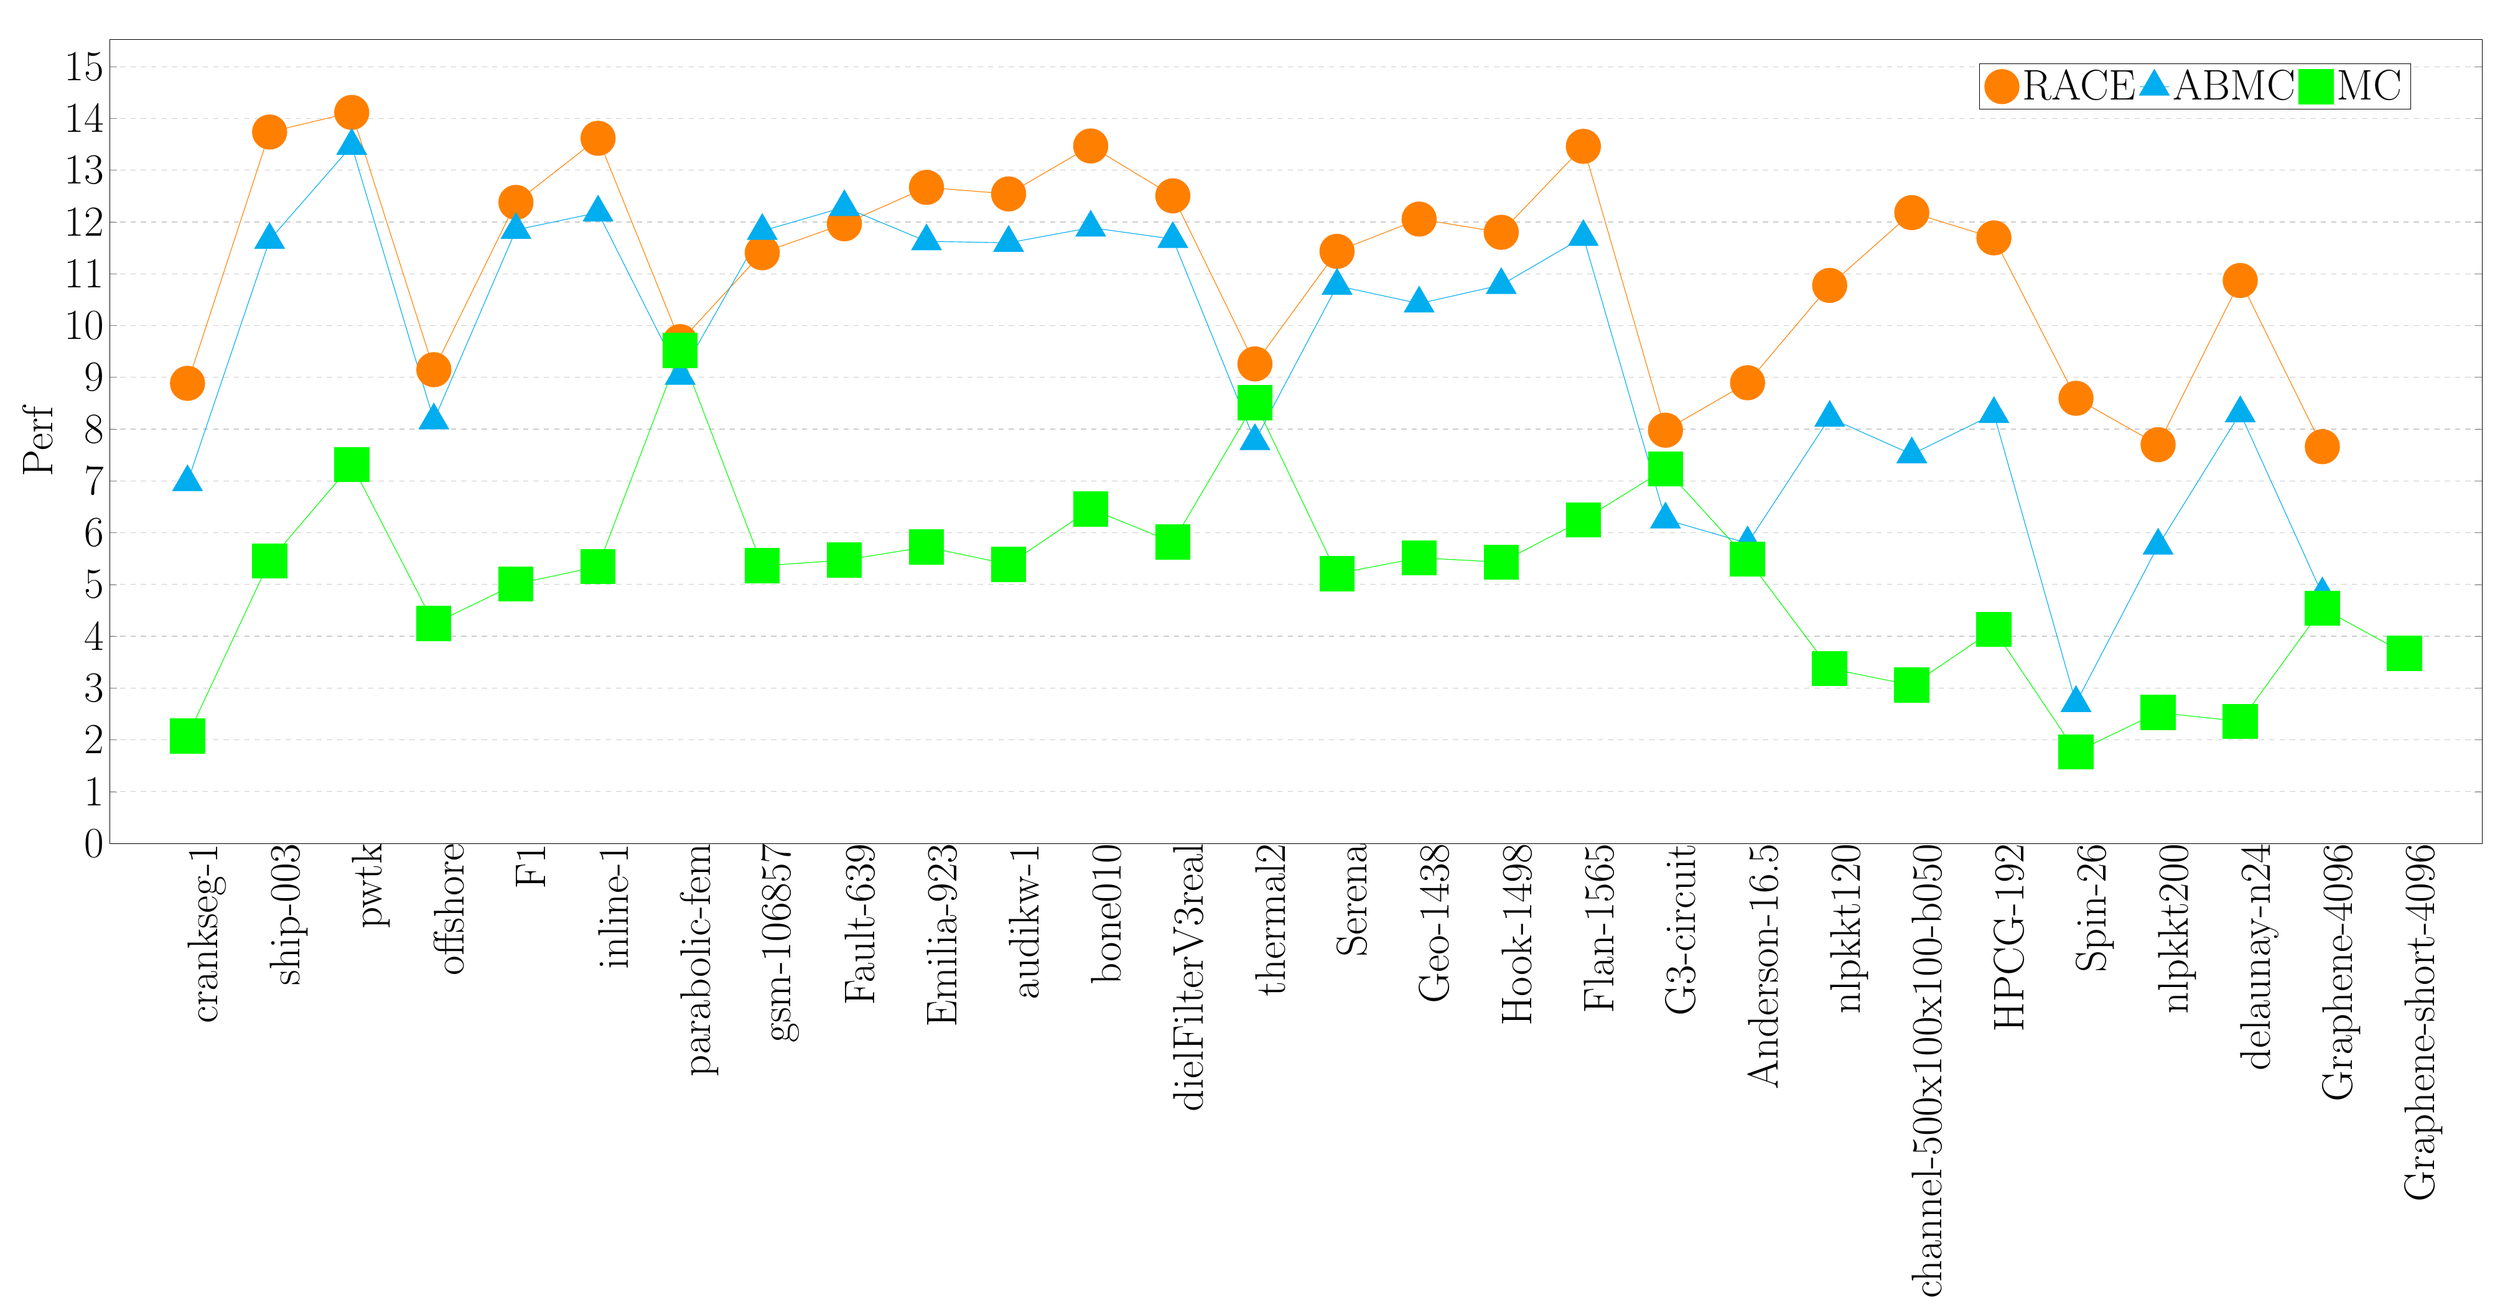
\begin{tikzpicture}
		%	\node at (13.25,15) {\LARGE{}};
			\begin{axis}[
		%	xmin=0.25, xmax=7.25,
			ymin=0, %ymax=3.25,
			xtick={1, 2, 3, 4, 5, 6, 7, 8, 9, 10, 11, 12, 13, 14, 15, 16, 17, 18, 19, 20, 21, 22, 23, 24, 25, 26, 27, 28},
		%	ytick={0,0.5,1,1.5,2,2.5,3},
			xticklabels={crankseg-1, ship-003, pwtk, offshore, F1, inline-1, parabolic-fem, gsm-106857, Fault-639, Emilia-923, audikw-1, bone010, dielFilterV3real, thermal2, Serena, Geo-1438, Hook-1498, Flan-1565, G3-circuit, Anderson-16.5, nlpkkt120, channel-500x100x100-b050, HPCG-192, Spin-26, nlpkkt200, delaunay-n24, Graphene-4096, Graphene-short-4096},
			width  = 50cm,
			height = 18cm,
			major x tick style = transparent,
			%	minor ytick={1, 5, 10, 15, 20, 25, 30 ,35,40},
			grid = minor,	
			%add_bar_commands
			ymajorgrids = true,
			grid style={dashed, gray!40},
			ylabel = {\Huge{Perf}},
		%	symbolic x coords={Graphene-2048-2048, Graphene-4096-4096, Spin-24-24-24},
			x tick label style={rotate=90, anchor=north east, inner sep=0mm, font={\Huge}},
			tick label style={font={\Huge}},
			scaled y ticks = false,
			enlarge x limits=0.035,
			legend cell align=left,
			legend style={font=\Huge},
			legend columns=-1,
			legend style={
				%at={(1,1.05)},
				%anchor=south east,
				%column sep=1ex,
				legend pos=north east
			},
			%spl_legend_code
			title= {\Huge\scalebox{1.5}{{}}}
			]

\addplot[mark=*, mark size=10pt, mark options={orange}, draw=orange ] plot coordinates{(1,8.884432) (2,13.738199) (3,14.116591) (4,9.148223) (5,12.379258) (6,13.617325) (7,9.691272) (8,11.406291) (9,11.966174) (10,12.669137) (11,12.542886) (12,13.469159) (13,12.505755) (14,9.259474) (15,11.433692) (16,12.056546) (17,11.801897) (18,13.461479) (19,7.979641) (20,8.896093) (21,10.775755) (22,12.181725) (23,11.693850) (24,8.595671) (25,7.700053) (26,10.870611) (27,7.661424)};
\addplot[mark=triangle*, mark size=10pt, mark options={cyan}, draw=cyan ] plot coordinates{(1,6.975072) (2,11.654730) (3,13.470981) (4,8.168161) (5,11.847441) (6,12.182863) (7,9.030775) (8,11.827959) (9,12.287738) (10,11.627419) (11,11.598877) (12,11.891430) (13,11.672224) (14,7.769063) (15,10.768905) (16,10.425632) (17,10.783511) (18,11.710633) (19,6.256020) (20,5.794948) (21,8.218445) (22,7.513928) (23,8.291422) (24,2.710502) (25,5.750556) (26,8.306818) (27,4.808545)};
\addplot[mark=square*, mark size=10pt, mark options={green}, draw=green ] plot coordinates{(1,2.071782) (2,5.456925) (3,7.316592) (4,4.244834) (5,5.009281) (6,5.348364) (7,9.518131) (8,5.361370) (9,5.469871) (10,5.726142) (11,5.388325) (12,6.458304) (13,5.817631) (14,8.512979) (15,5.208055) (16,5.514765) (17,5.430896) (18,6.248868) (19,7.232466) (20,5.490066) (21,3.376530) (22,3.055118) (23,4.131478) (24,1.767343) (25,2.526530) (26,2.356304) (27,4.539848) (28,3.671535)};
	%addplot cmd

	\legend{RACE, ABMC, MC}

	\end{axis}			
\end{tikzpicture}

\end{document}

